\documentclass[a4paper, 11pt]{scrartcl}
\usepackage[a4paper,left=3cm,right=2.5cm,top=2cm,bottom=2cm]{geometry}
\usepackage[ngerman]{babel}
\usepackage[T1]{fontenc}
\usepackage[utf8]{inputenc}
\usepackage{times}
\usepackage[onehalfspacing]{setspace}
\usepackage{graphicx}
\usepackage[backend=bibtex]{biblatex}
\usepackage{csquotes}
\usepackage{hyperref}
\usepackage{caption}
\usepackage{float}
\usepackage[headsepline, automark, nouppercase, singlespacing=true]{scrlayer-scrpage}

%-------------------------------------------------------------------------------
% Settings
%---------------------------------------------------------------

\pagestyle{scrheadings}
\clearpairofpagestyles
\ihead*{\headmark}
\ofoot*{\pagemark}
\renewcommand*{\headfont}{\normalfont}
\renewcommand*{\sectionmarkformat}{}
\setlength{\headheight}{14.5pt}
\relax
%change title of tableofcontents
\addto\captionsngerman{\renewcommand{\contentsname}{Inhalt}}
%remove biblatex warnings
\nocite{*}
%add bibliography
\addbibresource{bibliography.bib}
% change indent of toc to 0em
\RedeclareSectionCommand[tocindent=0em]{section}
\RedeclareSectionCommand[tocindent=0em]{subsection}
\RedeclareSectionCommand[tocindent=0em]{subsubsection}

%-------------------------------------------------------------------------------
% TITLE PAGE
%---------------------------------------------------------------

\title{ \normalsize \textbf{Dokumentation}
    \\2022 / 2023
    \leavevmode\\ [2.0cm]
    \hrule
    \leavevmode\\ [0.5cm]
    \LARGE \textbf{\uppercase{Versuch Switchkonfiguration}}
    \leavevmode\\ [1cm] 
    \hrule
    \leavevmode\\ [2cm] 
    \begin{center}
    
\includegraphics[scale=0.6]{bszet-lgo.png}
    \end{center}
	\normalsize  \vspace*{4.7\baselineskip}
    } 
\date{}
\author{
    Bonjov Hima \\
    Bjarne Doench \\
    Marius Starke \\ \\
    Betreut durch: Herr Ränsch}

%-------------------------------------------------------------------------------
% Main Content
%---------------------------------------------------------------

\begin{document}

    \pagenumbering{gobble}
    \maketitle

    \newpage
    \setcounter{page}{1}

    \pagenumbering{Roman}
    \tableofcontents
    \thispagestyle{scrheadings}
    \newpage

    \pagenumbering{arabic}
    \section{Projektbschreibung}

"All set up and ready to go? Let`s review some baseic concepts.
More interesting things to say here." \cite*{testbuch1}

    \newpage
\section{Vorbereitung}

    \subsection{Begriffserklärung}

        \subsubsection{Switch-Stacking}

        Switch-Stacking ist ein wichtiges Merkmal von Netzwerk-Switches.
        Diese Switches können miteinander verbunden werden, um als 
        logische Einheit zu fungieren. Durch das Zusammenschalten weiterer Switche, wird die Netzwerkkapazität 
        dank der höheren Anzahl verfügbarer Ports, besserer Ausfallsicherheit und der Möglichkeit 
        Link-Aggregation zu betreiben, erheblich erhöht. 
        Switch-Stacking wird nur von stapelbaren Switches unterstützt. \\\\
        Switches in einem Stack können mittels DAC-Kabeln, optischen Transceiver oder Stacking-Kabeln verbunden werden. 
        Es gibt einen Stack-Master, der das Zentrum des Stack-Systems ist und die Konfigurationsdaten verwaltet. 
        Die anderen Switches im Stack werden als Stack-Slaves bezeichnet. 
        Der Stack-Master kann von Benutzern verwaltet werden, und falls er ausfällt, wird ein neuer Master-Switch unter den Slaves ausgewählt.\\\\
        Zusammenfassend lassen sich folgende Vorteile von Switch-Stacking erschließen:
        \begin{itemize}
            \item Verbesserung der Zuverlässigkeit und Flexibilität des Netzwerkes
            \item Erhöhung der Bandbreite und Vereinfachung der Vernetzung
            \item hohe Skalierbarkeit des Netzwerkes
        \end{itemize}

        \subsubsection{Switchkaskadierung}

        Kaskadierung ist die traditionelle Methode zum Verbinden mehrerer Ethernet-Switches 
        und umfasst verschiedene Methoden für unterschiedliche Netzwerktopologien.\\
        Durch die Verknüpfung mehrerer Switches können Benutzer mehrere Ports haben, 
        die jeden Switch miteinander verbinden, unabhängig voneinander konfiguriert 
        und als Gruppe verwaltet werden können. 
        In einem Kaskaden-Switch-Netzwerk sind Daisy-Chain-Topologie und 
        Sterntopologie zwei gängige Methoden. 

        \subsubsection{Spanning-Tree-Verfahren}

        Der Spanning-Tree-Algorithmus führt eine Reihe von Schritten aus, 
        um sicherzustellen, dass die Topologie schleifenfrei ist und das Ethernet ordnungsgemäß funktioniert:\\
        \begin{enumerate}
            \item Root-Bridge-Auswahl – Zuerst wählt STP eine Root-Bridge aus. Dies ist der wichtigste Schalter in der Topologie. Es ist die Wurzel des azyklischen Baums.
            \item Schleifentopologie-Erkennung – Sobald die Root-Bridge ausgewählt ist, beginnt sie mit dem Senden von Spanning-Tree-Nachrichten (BPDUs). Der Switch verwendet diese Nachrichten, um den Teil der Topologie zu finden, der die Schleife enthält.
            \item Bestimmen der Port-Rollen – Nach dem Bestimmen des Loop-Teils der Topologie platziert jeder Switch so viele Switch-Ports wie nötig, um sicherzustellen, dass die Topologie schleifenfrei ist.
            \item Dropout – Switches tauschen weiterhin Nachrichten aus, um die Verfügbarkeit von Links und Nachbarkontakten zu verfolgen. Wenn die Verbindung oder der Switch ausfällt, führt der Switch die Schritte 2 und 3 erneut aus, um sicherzustellen, dass die neue Topologie schleifenfrei ist.
        \end{enumerate}

        \subsubsection{Auto-Negoatiation}

        Auto-Negotiation ist eine Funktion, die es zwei Netzwerken mit unterschiedlichen Geschwindigkeiten
        ermöglicht, zu kommunizieren und sich an eine Geschwindigkeit anpasst, 
        die für beide Netzwerke geeignet ist. 
        Beispielsweise verfügt ein Switch über einen 1-Gbit/s-Port (Gigabit-Ethernet), 
        der mit einem 100-Mbit/s-Port (Fast Ethernet) an einem anderen Switch verbunden ist. 
        Die Portgeschwindigkeiten an beiden Enden müssen gleich sein, um eine Verbindung herzustellen. 
        Das Autonegotiation-Protokoll teilt Baudrate, Duplexmodusstatus und Flusssteuerungsinformationen zwischen zwei Ports. 
        Sobald der Port die obigen Parameterinformationen empfangen hat, 
        passt er seinen Pegel entsprechend den Fähigkeiten des Peer-Ports an.

        \subsubsection{AutoUplink(MDI/MDI-X)}

        Ein Ethernet-Netzwerkport (z. B. an einem Switch) verwendet die automatische Uplink-Funktion, um zu erkennen, 
        an welchen Switch er senden und empfangen (MDI/MDIX) soll. 
        Mit der automatischen Uplink-Funktion können sowohl Crossover-Kabel 
        als auch 1:1-Netzwerkkabel verwendet werden.

        \newpage
        \subsubsection{Link Aggregation/ Port Trunking}

        \newpage
        \subsubsection{Vollduplex-Betrieb}

        \newpage
        \subsubsection{Mac-Adressenfilter}

    \newpage
    \subsection{Netzwerktrennung}

        \subsubsection{VLAN}

        \newpage
        \subsubsection{VLAN-Tagging}

    \newpage
    \subsection{Übersicht des NETGEAR-Switches}
    
    \newpage
\section{Versuchsaufbau}

    \subsection{Szenario}

    Im ersten Schritt wurde das Netzwerk mithilfe von Subnetting getrennt und anschließend unter Verwendung von managebaren NETGEAR-Switches
    in unterschiedliche VLANs unterteilt.

    \subsection{Durchführung}

        \subsubsection{Funktionsprüfung des Netzwerks}
        \begin{table}[H]
            \centering
            \begin{tabular}{l|c|l|c|l|c|l|c|l|c|}
            \multicolumn{1}{l}{} & \multicolumn{1}{l}{PC1} & \multicolumn{1}{l}{PC2} & \multicolumn{1}{l}{PC3} & \multicolumn{1}{l}{PC4}  \\ 
            \cline{2-5}
            PC1&&X&& \\ 
            \cline{2-5}
            PC2&X&&& \\
            \cline{2-5}
            PC3&&&&X \\
            \cline{2-5}
            PC4&&&X& \\
            \cline{2-5}
            \end{tabular}
            \caption{Ergebnistabelle\\ (Erreichbarkeit der einzelnen PCs untereinander) mittels "`ping"'-command}
        \end{table}
        
        \subsubsection{Unterteilung in Subnetze}
        Im folgenden Screenshot ist unser Netzwerkplan dokumentiert, welcher als Grundlage für
        den Versuchsaufbau fungiert.
        \begin{figure}[H]
            \centering
            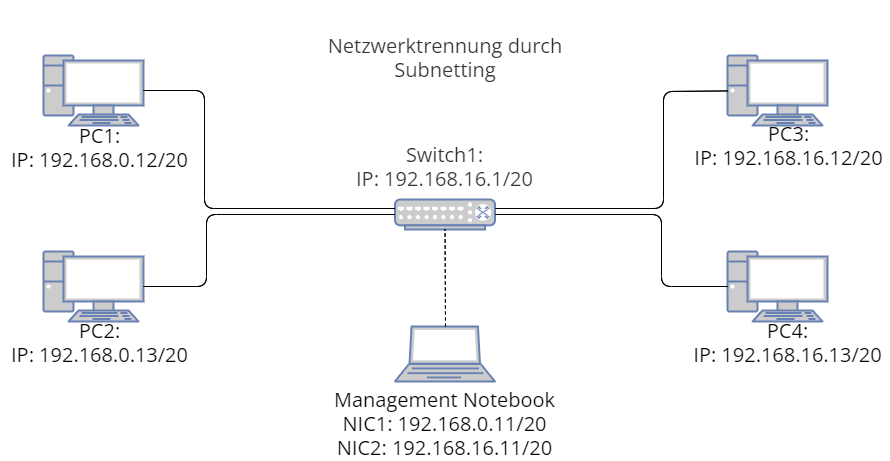
\includegraphics[scale=0.5]{images/Unterteilung in Subnetze/Netzwerkplan_Subnetting_new.png}
            \caption{Netzwerkplan Subnetting}
        \end{figure}
        Die beiden folgenden Screenshots zeigen, dass im Netzwerk zwei PCs erreichbar sind. Im ersten Netzwerk (192.168.0.0) 
        sind die Clients 1 und 2 mit den IP-Adressen 192.168.0.12 und 192.168.0.13 zu finden, während sich im zweiten Netzwerk 
        (192.168.16.0) die Clients 3 und 4 mit den IP-Adressen 192.168.16.12 und 192.168.16.13 befinden. Der Switch(192.168.16.1)
        befindet sich im zeiten Netzwerk(192.168.16.0).
        \begin{figure}[H]
        \centering
            \begin{subfigure}{.5\textwidth}
              \centering
              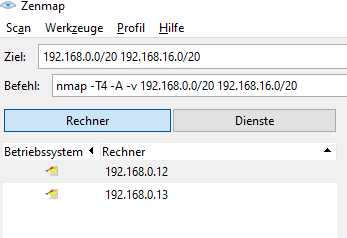
\includegraphics[scale=0.7]{images/Unterteilung in Subnetze/Scan_Subnetz_1.png}
              \caption{Subnetz 1 (192.168.0.0)}
            \end{subfigure}%
            \begin{subfigure}{.5\textwidth}
              \centering
              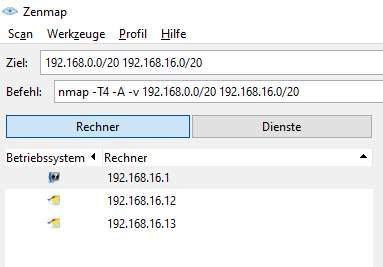
\includegraphics[scale=0.7]{images/Unterteilung in Subnetze/Scan_Subnetz_2.png}
              \caption{Subnetz 2 (192.168.16.0) mit Switch}
            \end{subfigure}
        \caption{Zenmap-Scan Subnetze}
        \end{figure}
        
        Es ist ersichtlich, dass die Clients der beiden Netzwerke nicht miteinander kommunizieren können, wodurch eine abteilungsübergreifende 
        Erreichbarkeit der PCs nicht mehr möglich ist. Dies ist auch in den beiden folgenden Screenshots deutlich erkennbar, 
        in denen der Befehl "`ipconfig"' und "`ping"' in der Befehlszeile des jeweiligen Clients ausgeführt wurde.
        
        \begin{figure}[H]
        \centering
            \begin{subfigure}{\textwidth}
                \centering
                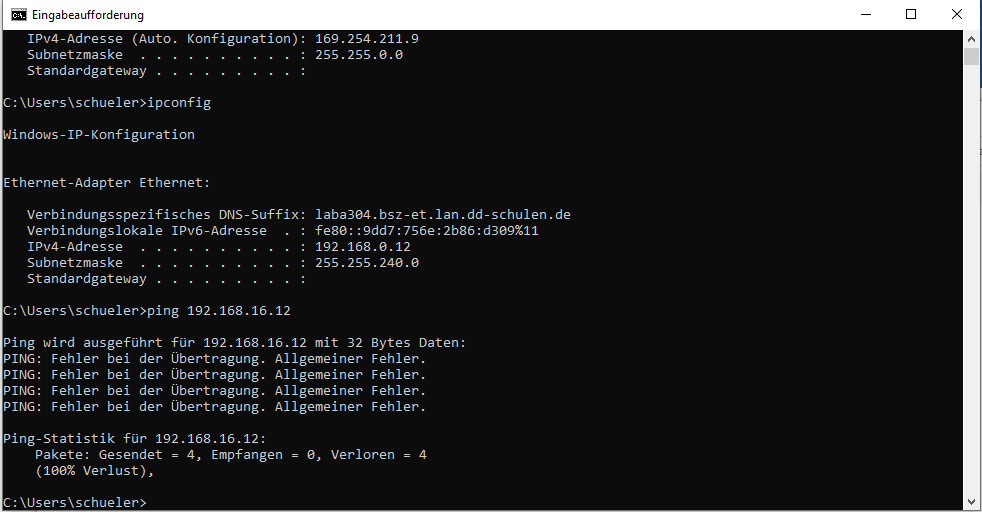
\includegraphics[scale=0.5]{images/Unterteilung in Subnetze/SubnetzPC1_PingPC3.png}
                \caption{ping PC1 zu PC3}
            \end{subfigure}
            \begin{subfigure}{\textwidth}
                \centering
                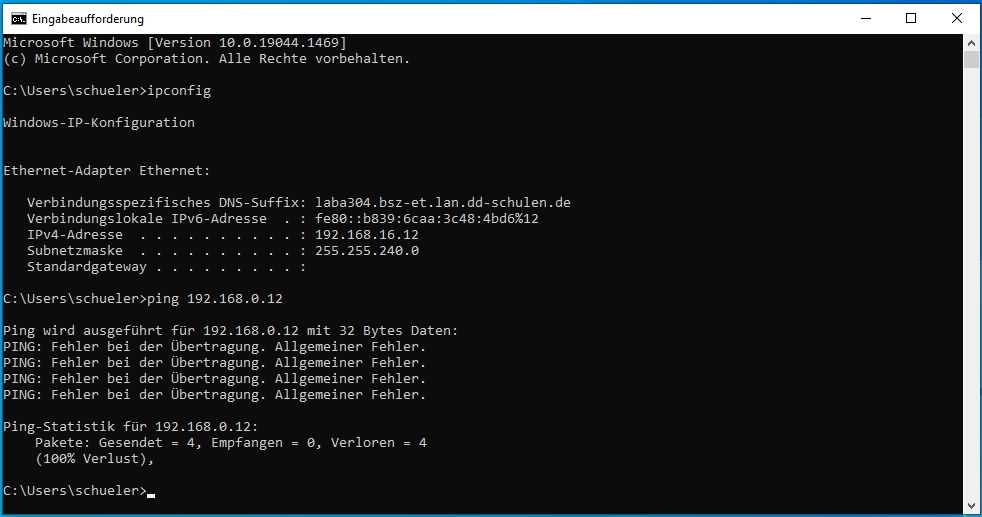
\includegraphics[scale=0.5]{images/Unterteilung in Subnetze/SubnetzPC3_PingPC1.png}
                \caption{ping PC3 zu PC1}
            \end{subfigure}
        \caption{Erreichbarkeit Netzwerke Subnetting}
        \end{figure}

        \newpage
        \subsubsection{Trennung durch VLAN herstellen}
        Im folgenden Screenshot ist unser Netzwerkplan dokumentiert, welcher als Grundlage für
        den Versuchsaufbau der Netzwertrennung durch VLANs fungiert.
        \begin{figure}[H]
            \centering
            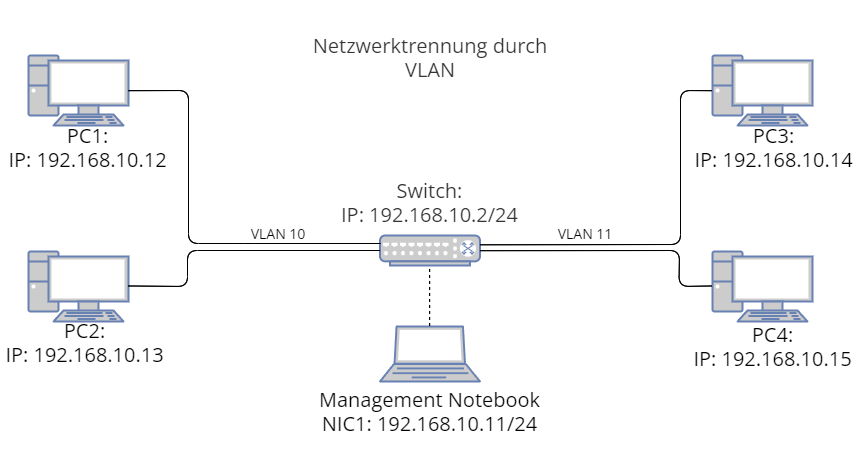
\includegraphics[width=\linewidth]{images/Trennung durch VLAN herstellen/Netzwerkplan_VLAN._portbasiert.png}
            \caption{Netzwerkplan portbasiertes VLAN}
        \end{figure}
        Um die Trennung durch VLANs zu realisieren haben wir als erstes ein portbasiertes VLAN eingerichtet, welches wir
        in den weiteren Aufgaben auf PVID erweitert haben.
        \begin{figure}[H]
        \centering
            \begin{subfigure}{\linewidth}
                \centering
                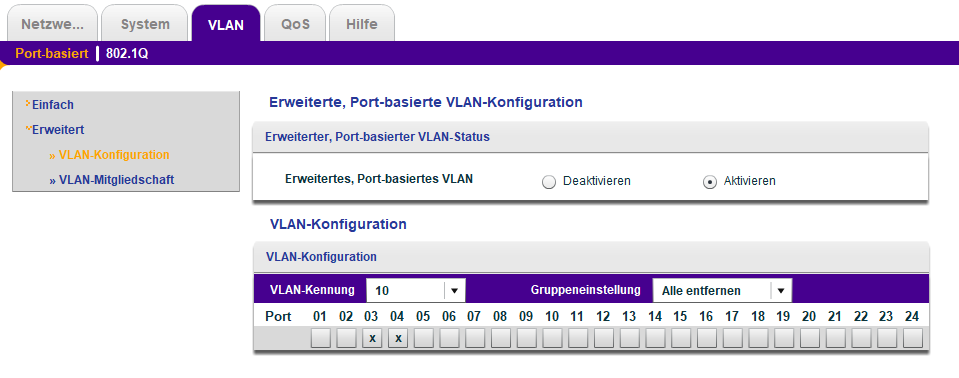
\includegraphics[scale=0.45]{images/Trennung durch VLAN herstellen/VLAN10_Konfiguration.png}
                \caption{VLAN10 Konfiguration}
            \end{subfigure}
            \begin{subfigure}{\linewidth}
                \centering
                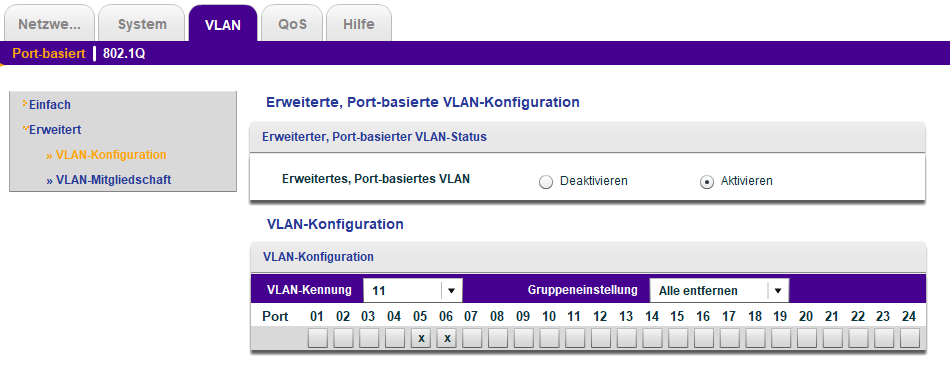
\includegraphics[scale=0.45]{images/Trennung durch VLAN herstellen/VLAN11_Konfiguration.png}
                \caption{VLAN11 Konfiguration}
            \end{subfigure}
        \caption{Konfiguration des portbasierten VLANs}
        \end{figure}

        \newpage
        Die Clients sind hierbei in zwei VLANs getrennt, 10 und 11. In den folgenden Screenshots sind Erreichbarkeiten
        der anderen Clients an dem jeweiligen Client dokumentiert.
        \begin{figure}[H]
        \centering
            \begin{subfigure}{.45\linewidth}
                \centering
                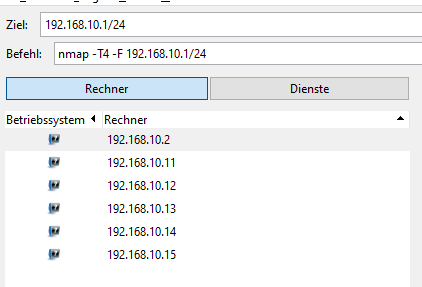
\includegraphics[width=\linewidth]{images/Trennung durch VLAN herstellen/ErreichbarkeitAnliegendAn11.png}
                \caption{Erreichbarkeit anliegend an Management Notebook}
            \end{subfigure}
            \begin{subfigure}{.45\linewidth}
                \centering
                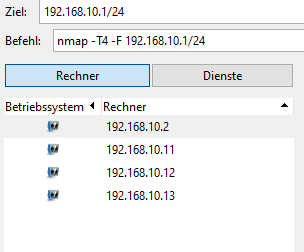
\includegraphics[width=\linewidth]{images/Trennung durch VLAN herstellen/ErreichbarkeitAnliegendAn12.png}
                \caption{Erreichbarkeit anliegend an PC1}
            \end{subfigure}
            \begin{subfigure}{\textwidth}
                \centering
                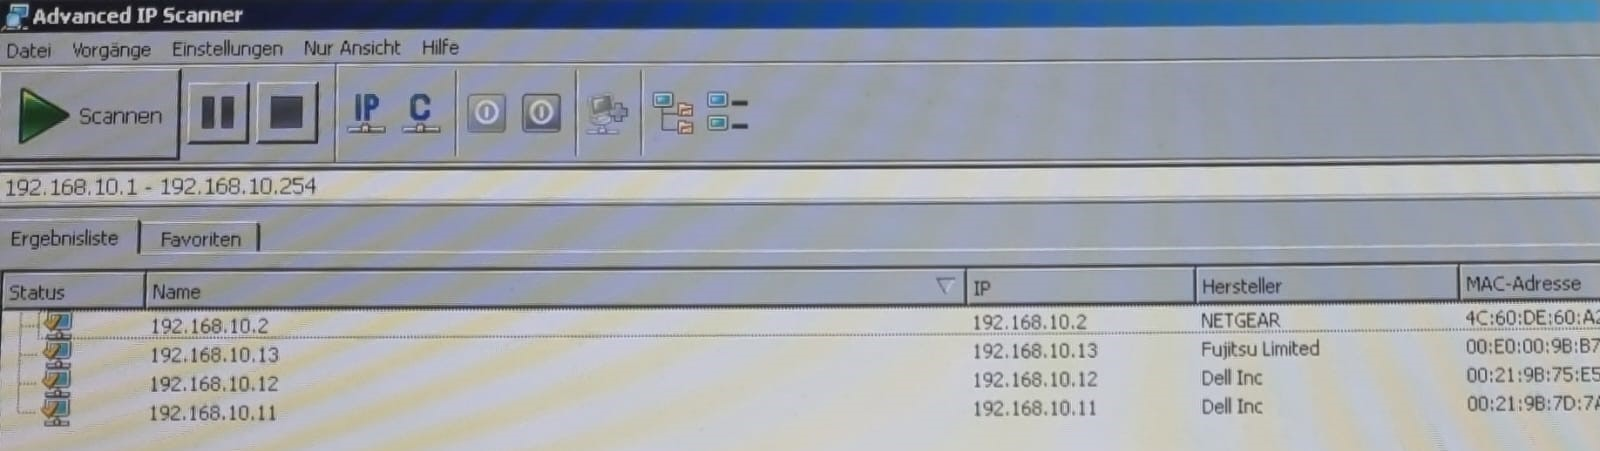
\includegraphics[width=\linewidth]{images/Trennung durch VLAN herstellen/ErreichbarkeitAnliegendAn13.jpg}
                \caption{Erreichbarkeit anliegend an PC2}
            \end{subfigure}
            \begin{subfigure}{\textwidth}
                \centering
                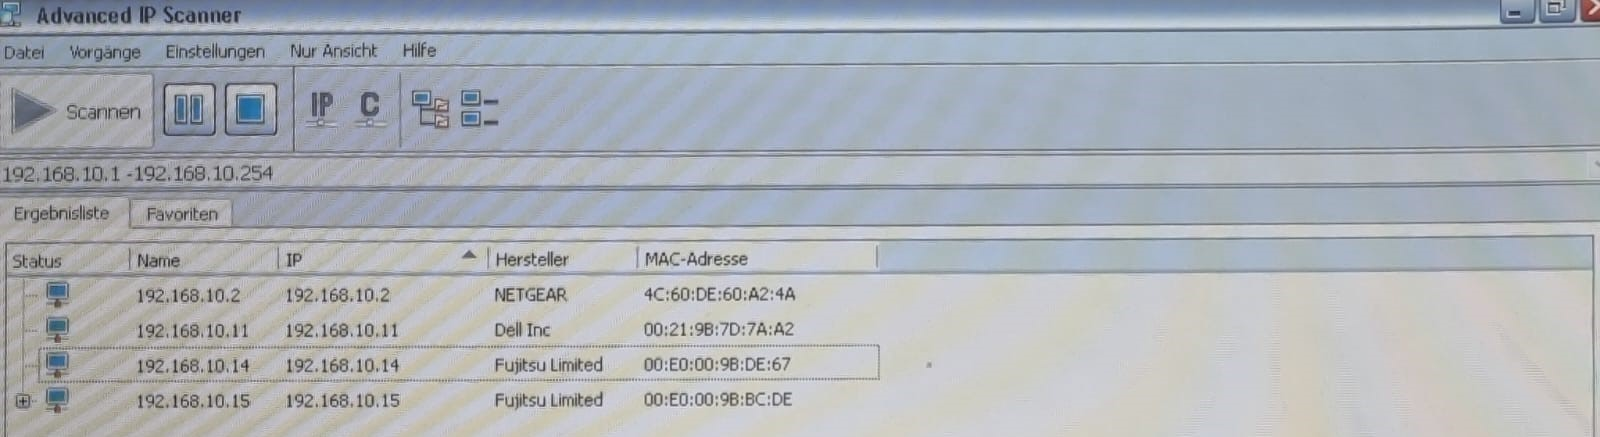
\includegraphics[width=\linewidth]{images/Trennung durch VLAN herstellen/ErreichbarkeitAnliegendAn14.jpg}
                \caption{Erreichbarkeit anliegend an PC3}
            \end{subfigure}
            \begin{subfigure}{\textwidth}
                \centering
                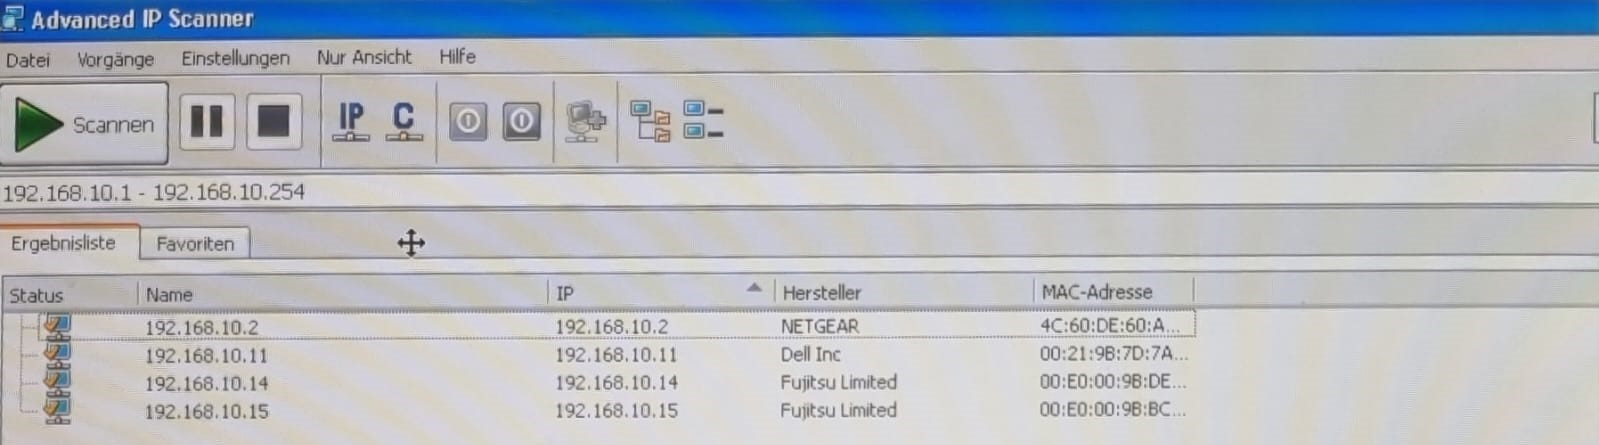
\includegraphics[width=\linewidth]{images/Trennung durch VLAN herstellen/ErreichbarkeitAnliegendAn15.jpg}
                \caption{Erreichbarkeit anliegend an PC4}
            \end{subfigure}
        \caption{Erreichbarkeiten im portbasierten VLAN}
        \end{figure}
        Aus den oben aufgezeigten Screenshots lässt sich erkennen, dass ausschließlich die Clients der 
        zugehörigen VLANs miteinander kommunizieren können.


        \newpage
        \subsubsection{VLAN übergreifenden Server integrieren}
        Um einen VLAN-übergreifenden Server zu integrieren, ist es erforderlich, ein zusätzliches VLAN einzubeziehen, 
        das die Verbindung zwischen den VLANs herstellt, jedoch keine direkte Kommunikation ermöglicht. Im folgenden Netzwerkplan 
        wird mithilfe des Management-Notebooks die Realisierung eines neuen VLANs 12 erreicht, wobei die Mitglieder von VLAN 10 und 11 
        ebenfalls Teil von VLAN 12 sind.
        \begin{figure}[H]
            \centering
            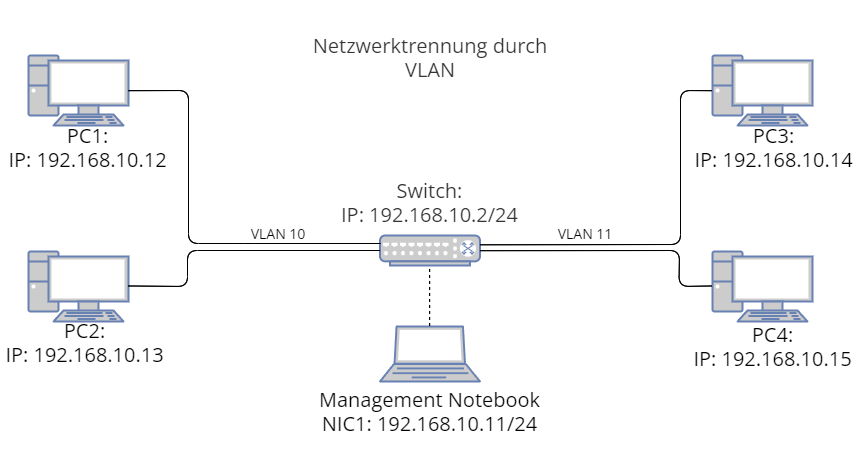
\includegraphics[width=\linewidth]{images/Trennung durch VLAN herstellen/Netzwerkplan_VLAN._portbasiert.png}
            \caption{Netzwerkplan - Integration eines Servers}
        \end{figure}
        Der nächste Screenshot dokumentiert die Konfiguration des Switches zur Einrichtung des VLAN 12.
        Hierbei haben wir von portbasiertem VLAN auf die erweiterte 802.1Q-VLAN-Konfiguration umgestellt.
        \begin{figure}[H]
            \centering
            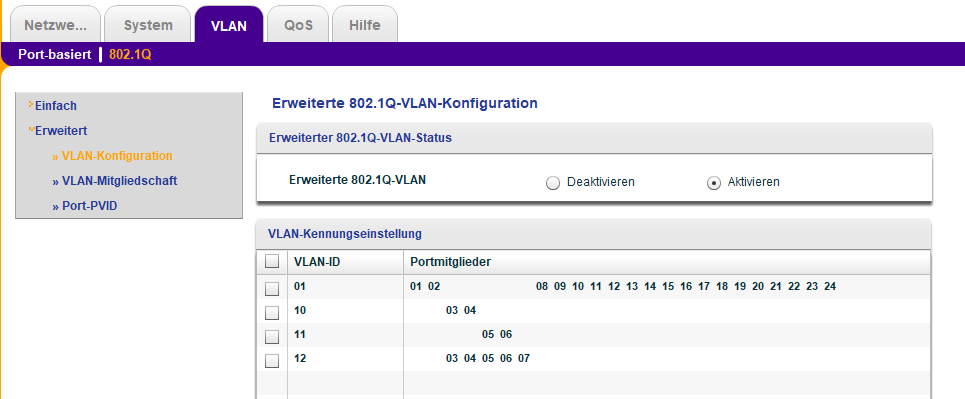
\includegraphics[width=\linewidth]{images/VLAN übergreifenden Server integrieren/VlanKonfigurationMitServer.png}
            \caption{Switch Konfiguration - Integration eines Servers}
        \end{figure}
        \begin{figure}[H]
        \centering
            \begin{subfigure}{\linewidth}
                \centering
                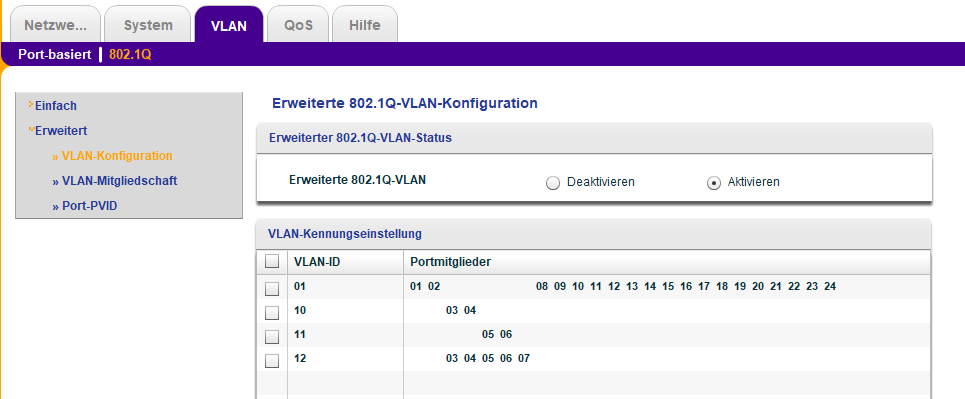
\includegraphics[width=\linewidth]{images/VLAN übergreifenden Server integrieren/VlanKonfigurationMitServer.png}
                \caption{Übersicht der VLAN-Mitgliedschaften}
            \end{subfigure}
            \begin{subfigure}{.49\linewidth}
                \centering
                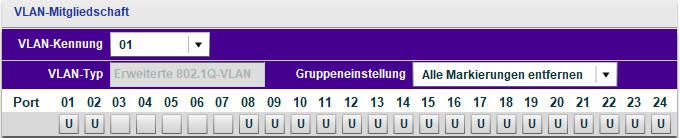
\includegraphics[width=\linewidth]{images/VLAN übergreifenden Server integrieren/VlanMitgliedschaft1.png}
                \caption{VLAN01 - Mitgliedschaften}
            \end{subfigure}
            \begin{subfigure}{.49\linewidth}
                \centering
                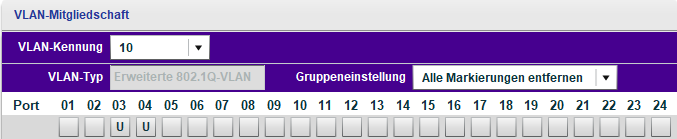
\includegraphics[width=\linewidth]{images/VLAN übergreifenden Server integrieren/VlanMitgliedschaft2.png}
                \caption{VLAN10 - Mitgliedschaften}
            \end{subfigure}
            \begin{subfigure}{.49\linewidth}
                \centering
                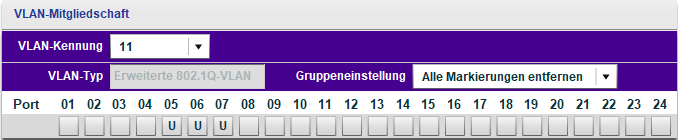
\includegraphics[width=\linewidth]{images/VLAN übergreifenden Server integrieren/VlanMitgliedschaft3.png}
                \caption{VLAN11 - Mitgliedschaften}
            \end{subfigure}
            \begin{subfigure}{.49\linewidth}
                \centering
                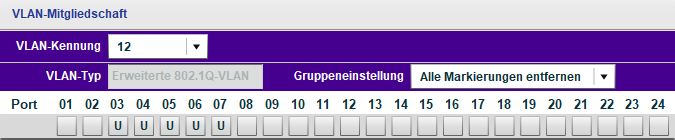
\includegraphics[width=\linewidth]{images/VLAN übergreifenden Server integrieren/VlanMitgliedschaft4.png}
                \caption{VLAN12 - Mitgliedschaften}
            \end{subfigure}
        \caption{Switch Konfiguration - Integration eines Servers}
        \end{figure}
        \begin{figure}[H]
            \centering
            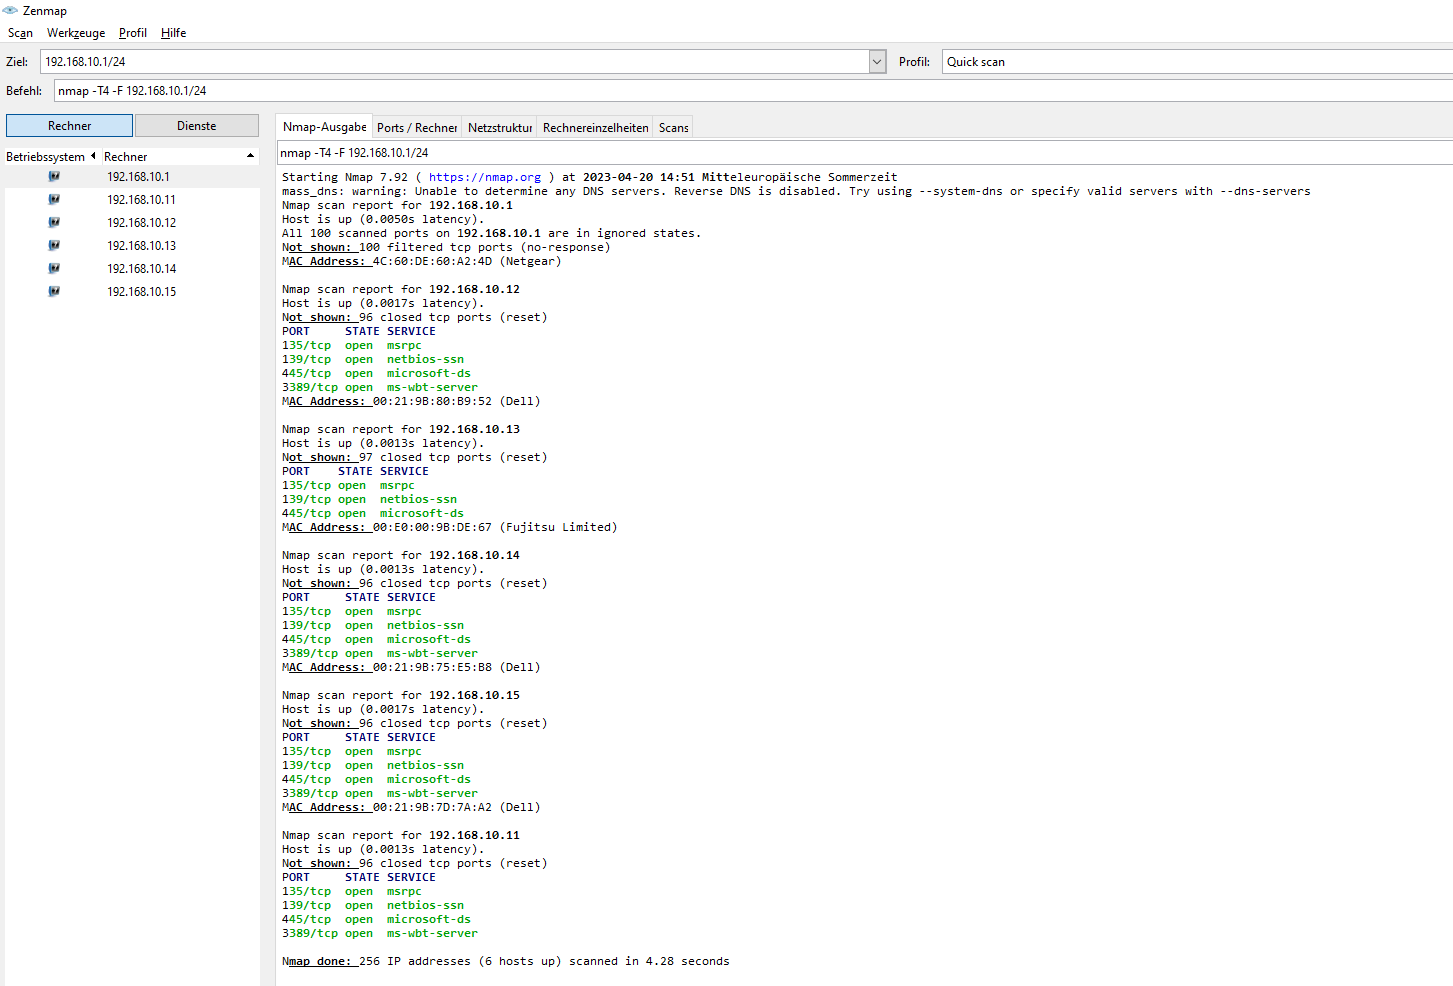
\includegraphics[width=\linewidth]{images/VLAN übergreifenden Server integrieren/serverVLAN12_IP11.png}
            \caption{Zenmap-Scan Server - Integration eines Servers}
        \end{figure}

        \newpage
        \subsubsection{Einrichtung Layer2-Switche}
        Da wir sowohl einen weiteren Switch als auch neue Clients zur Integration der neuen Abteilung benötigten, 
        mussten wir zunächst einen neuen Netzwerkplan erstellen, in welchem die Verbindung mit einem Layer2-Switch ermöglicht wird.
        Hierbei haben wir den zweiten Switch mittels eines Trunking-Ports nach dem Switch-Stacking Verfahren an den ersten Switch angebunden.
        \begin{figure}[H]
            \centering
            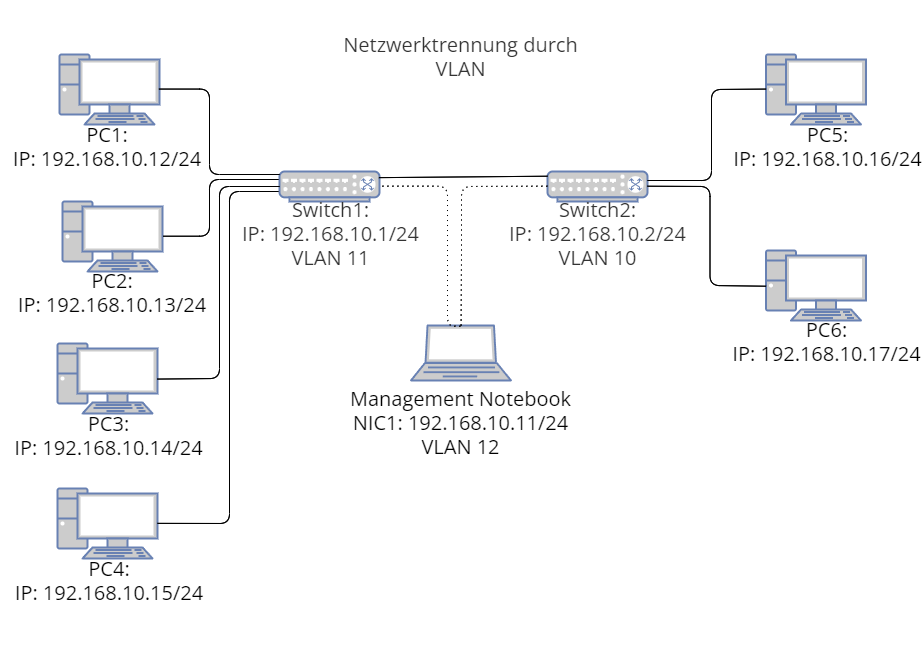
\includegraphics[width=\linewidth]{images/Einrichtung Layer2-Switche/Netzwerkplan_VLAN_switch_stacking.png}
            \caption{Netzwerkplan - Layer2-Switche}
        \end{figure}
        Unser Versuchsaufbau mit dem hinzugefügten Switch, der über Port1 mit dem ersten Switch verbunden ist, sah wie folgt aus:
        \begin{figure}[H]
            \centering
            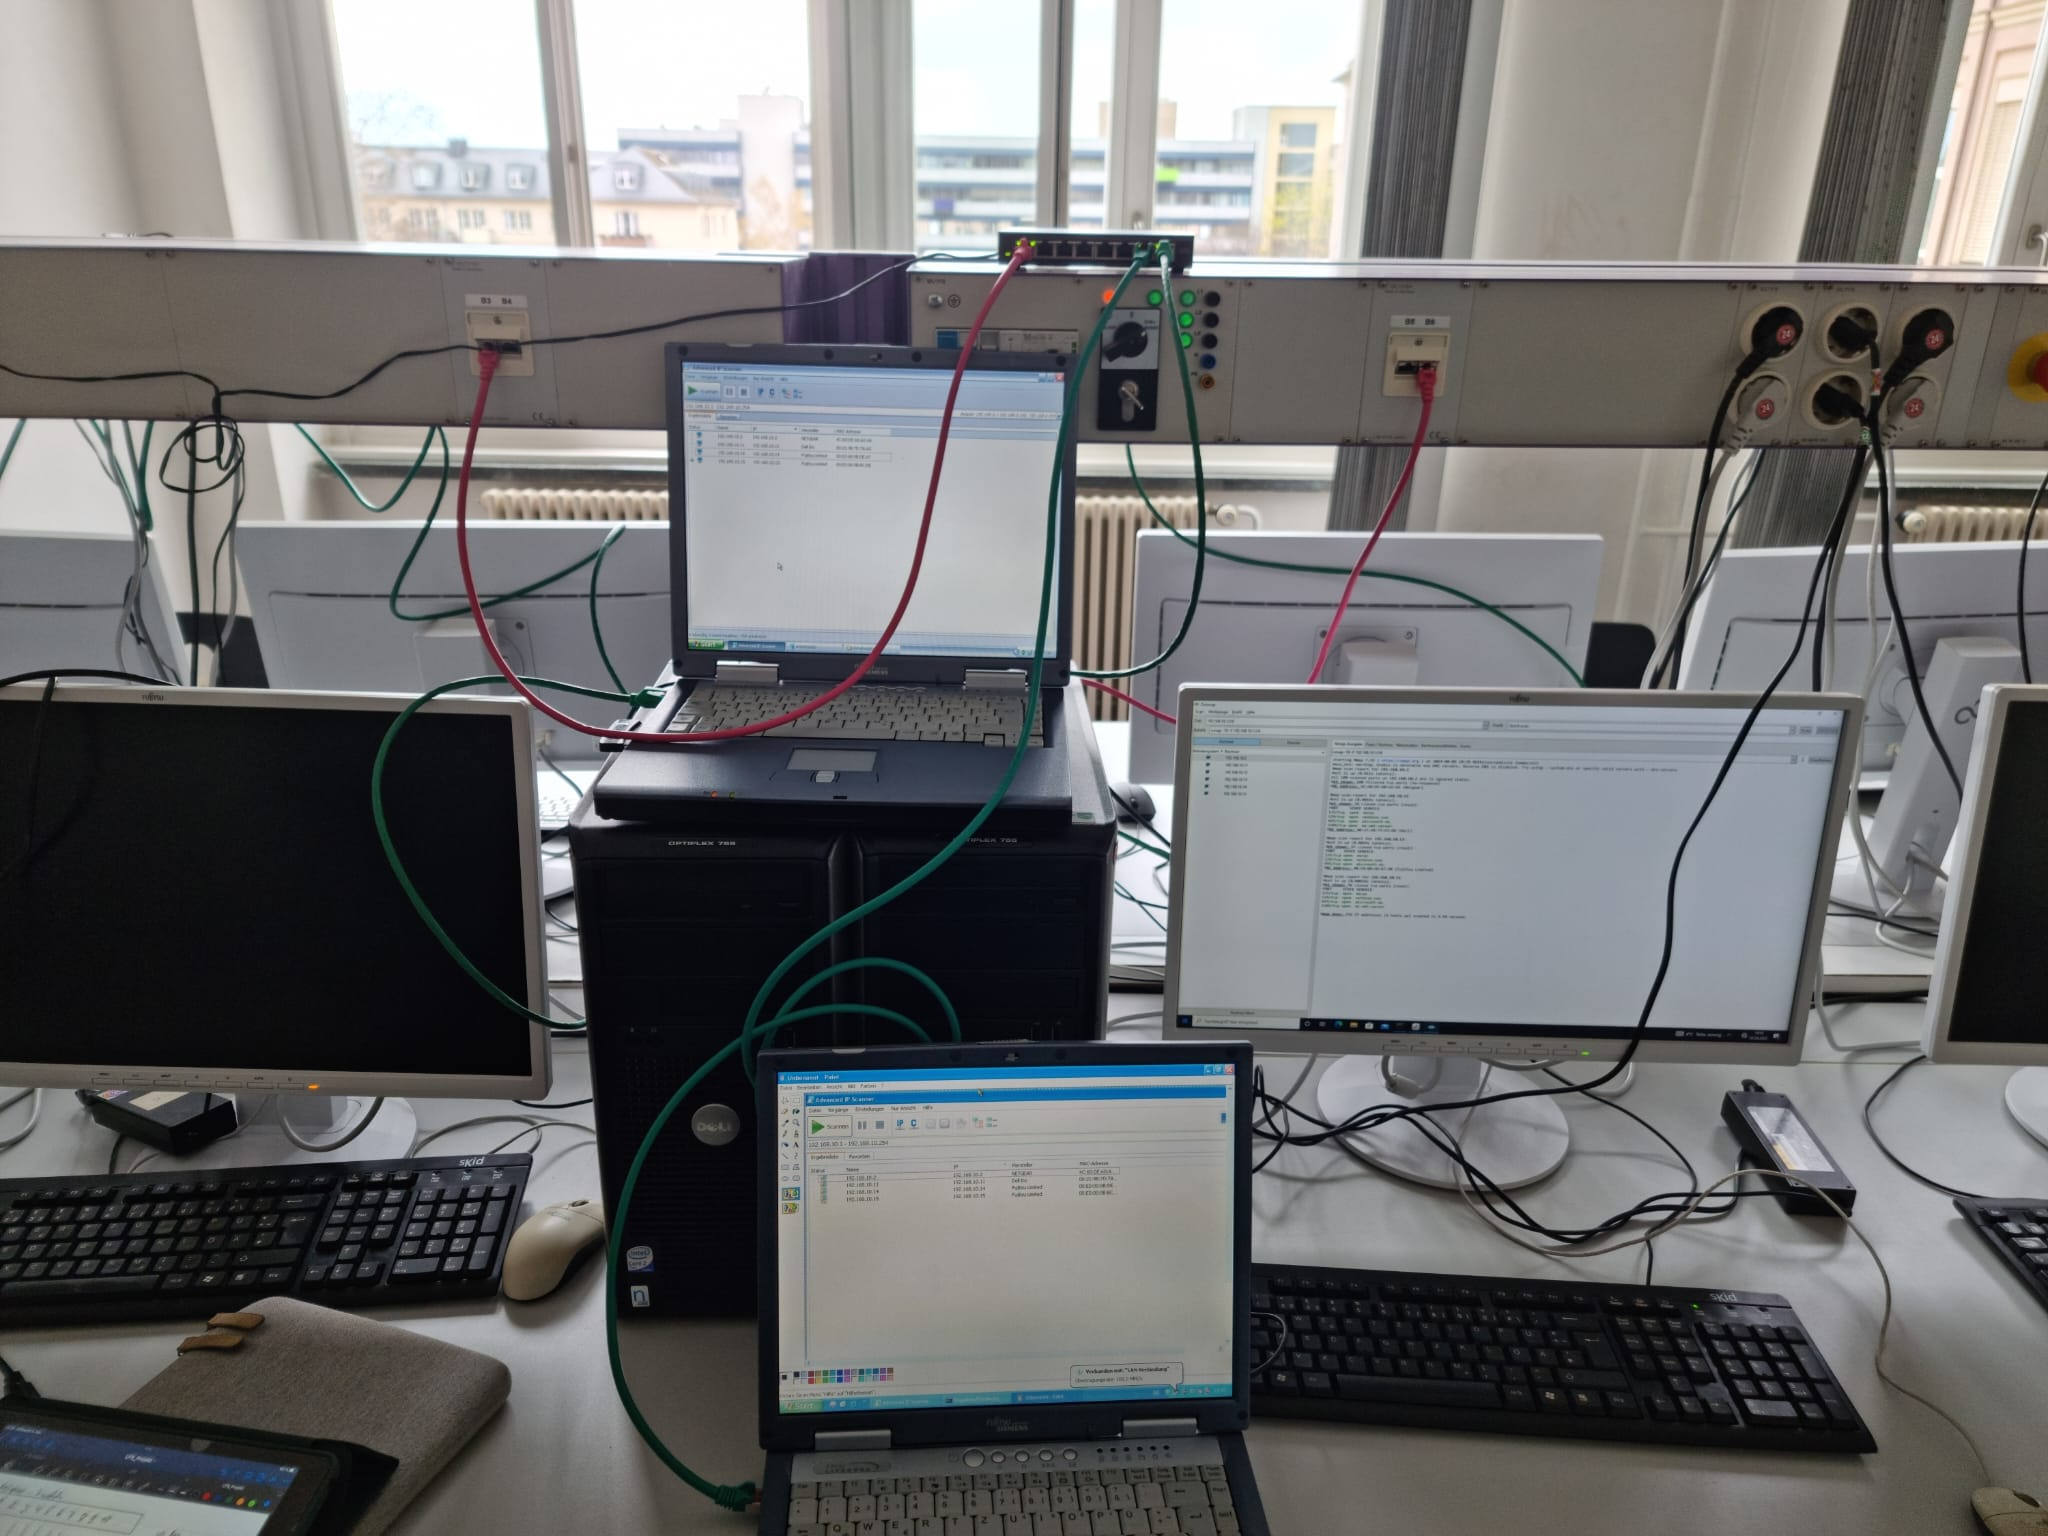
\includegraphics[width=0.6\linewidth]{images/Einrichtung Layer2-Switche/AufbauVersuch.jpg}
            \caption{Versuchsaufbau - Layer2-Switche}
        \end{figure}
        Des weiteren mussten wir die Konfiguration der Switche verändern:
        \begin{figure}[H]
        \centering
            \begin{subfigure}{.49\linewidth}
                \centering
                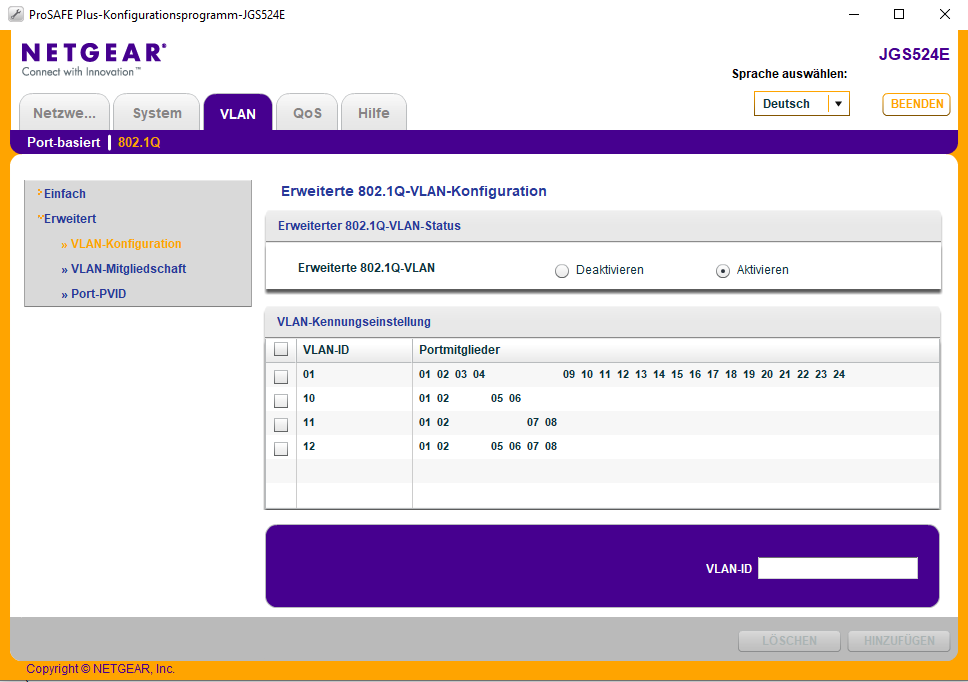
\includegraphics[width=\linewidth]{images/Einrichtung Layer2-Switche/Config_Switch1.png}
                \caption{Mitgliedschaften Switch1}
            \end{subfigure}
            \begin{subfigure}{.49\linewidth}
                \centering
                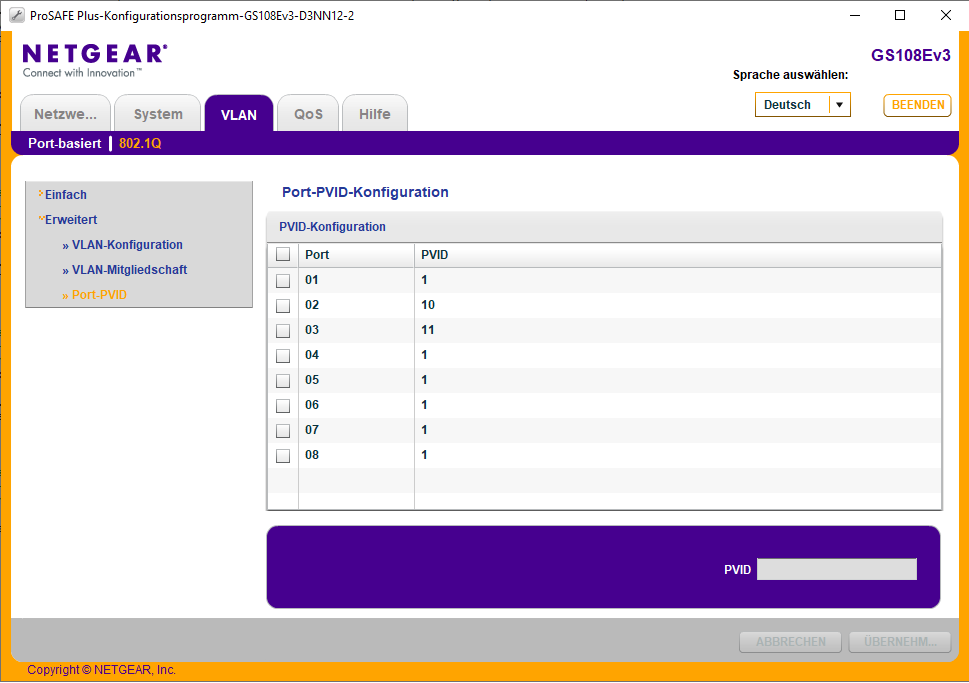
\includegraphics[width=\linewidth]{images/Einrichtung Layer2-Switche/Config_PortPVID_Switch2.png}
                \caption{PVID Switch1}
            \end{subfigure}
            \begin{subfigure}{.49\linewidth}
                \centering
                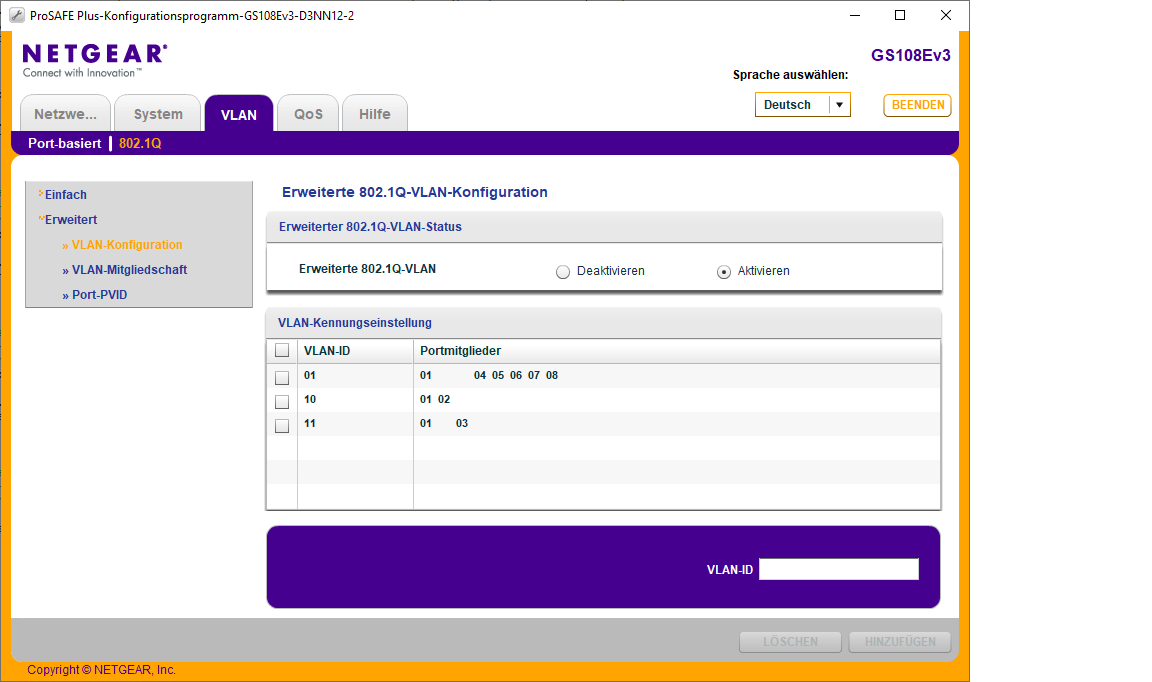
\includegraphics[width=\linewidth]{images/Einrichtung Layer2-Switche/Config_Switch2.png}
                \caption{Mitgliedschaften Switch2}
            \end{subfigure}
            \begin{subfigure}{.49\linewidth}
                \centering
                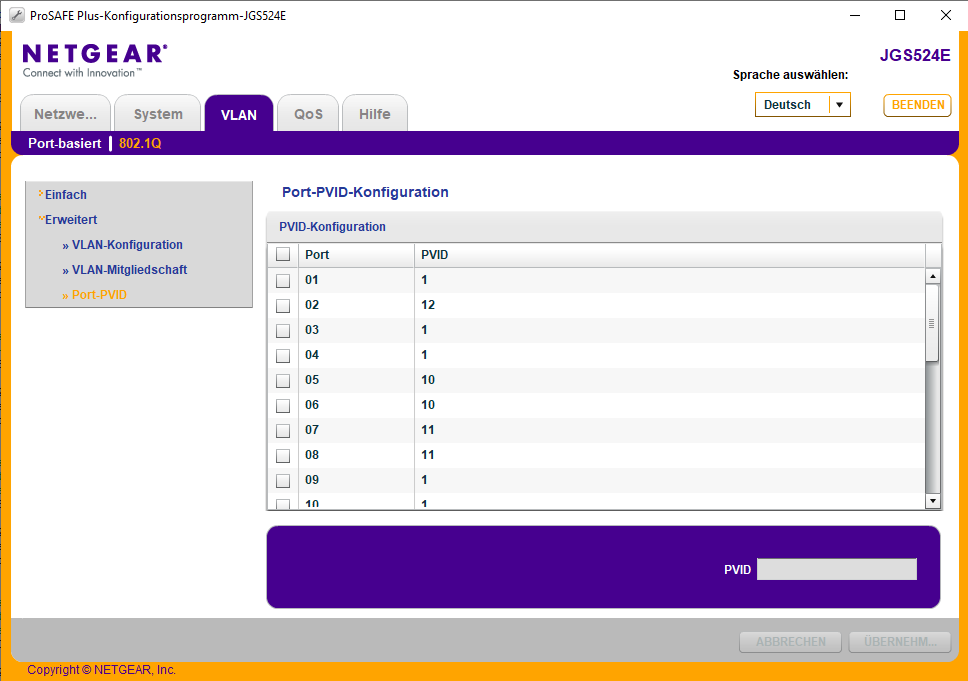
\includegraphics[width=\linewidth]{images/Einrichtung Layer2-Switche/Config_PVID_Switch1.png}
                \caption{PVID Switch2}
            \end{subfigure}
        \caption{Switch Konfiguration - Layer2-Switche}
        \end{figure}
         
        Um eine Kommunikation innerhalb der VLANs über mehrere Switches hinweg zu 
        ermöglichen, werden auf beiden Switches auf Port 1 Datenpakete mit 
        VLAN-Informationen verschickt, die als getaggte Pakete bezeichnet werden.
        Nach folgendem Schema habe wir die Portkonfiguration der Switche durchgeführt, 
        "`T"' steht in diesem Fall für "`Tagged"' und "`U"' für "`Untagged"'.
        \begin{figure}[H]
            \centering
            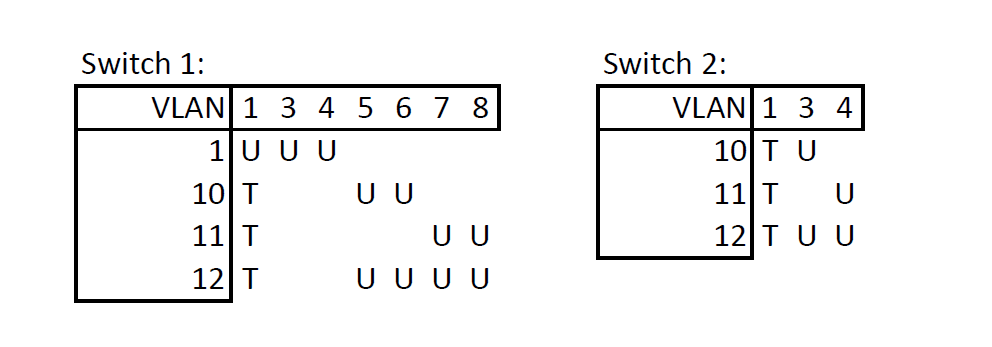
\includegraphics[width=\linewidth]{images/Einrichtung Layer2-Switche/Schema_SwitchKonfiguration_Tagged_untagged.png}
            \caption{Schema Switche - Layer2-Switche}
        \end{figure}
        \newpage
        Im Folgenden wird ersichtlich, dass nur die Clients im jeweiligen VLAN miteinander kommunizieren können:
        \begin{figure}[H]
        \centering
            \begin{subfigure}{\linewidth}
                \centering
                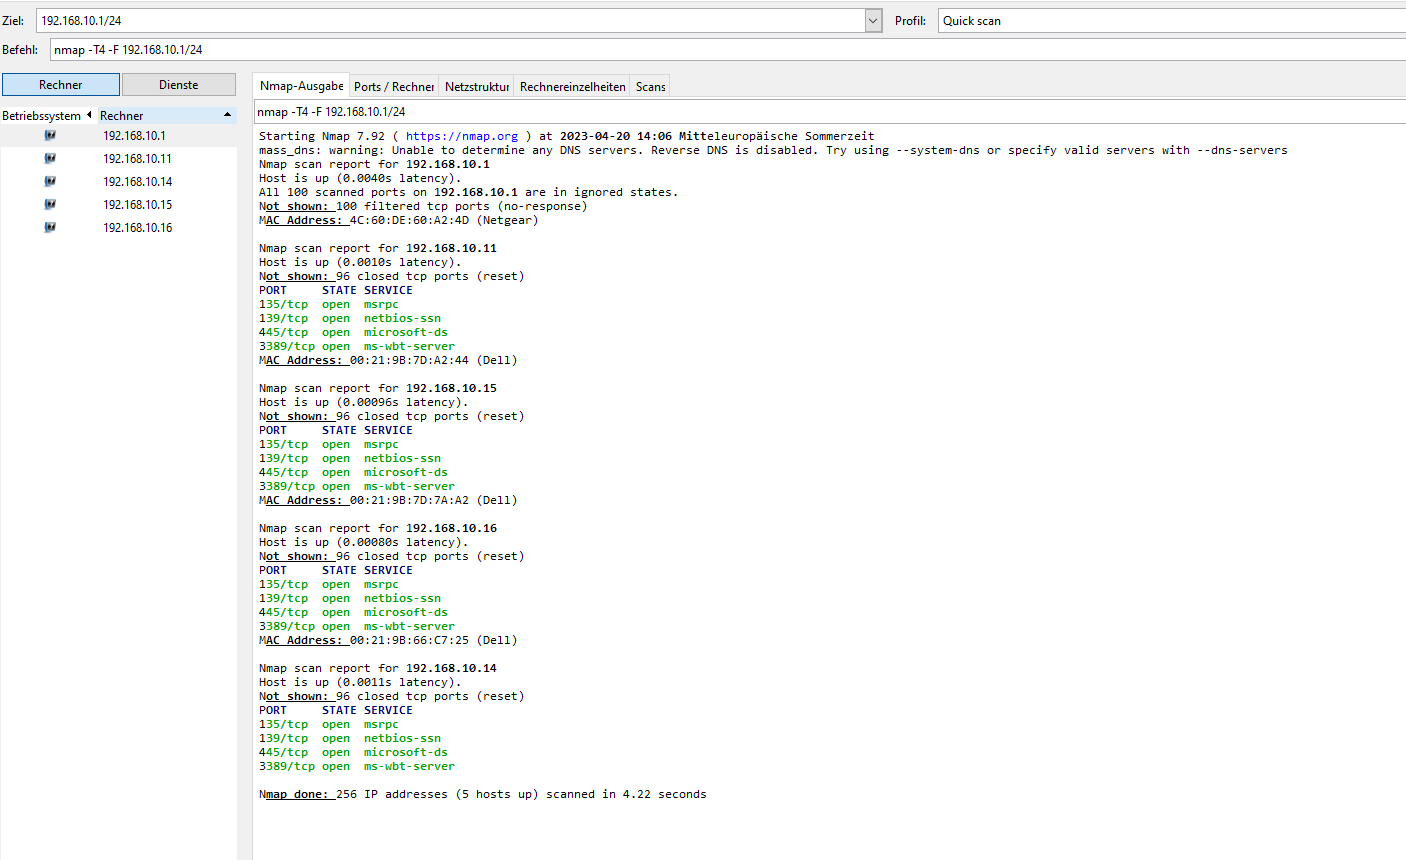
\includegraphics[width=\linewidth]{images/Einrichtung Layer2-Switche/ServerVLAN10Client14.png}
                \caption{Verbindungen Client 14}
            \end{subfigure}
            \begin{subfigure}{\linewidth}
                \centering
                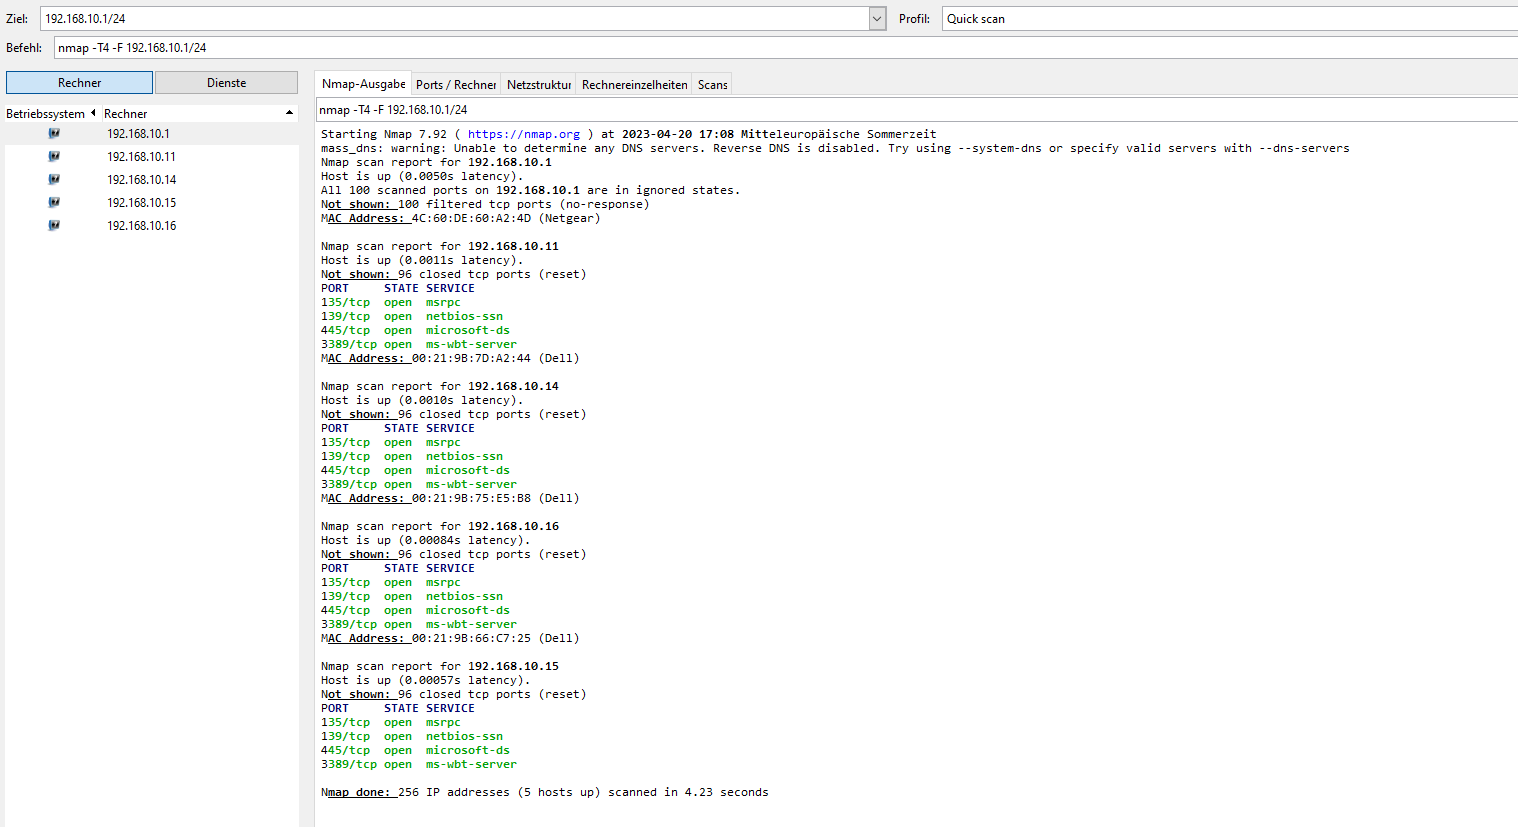
\includegraphics[width=\linewidth]{images/Einrichtung Layer2-Switche/ServerVLAN10Client15.png}
                \caption{Verbindungen Client 15}
            \end{subfigure}
        \caption{Verbindungen VLAN10 - Layer2-Switche}
        \end{figure}%
        \begin{figure}[H]\ContinuedFloat
        \centering
            \begin{subfigure}{\linewidth}
                \centering
                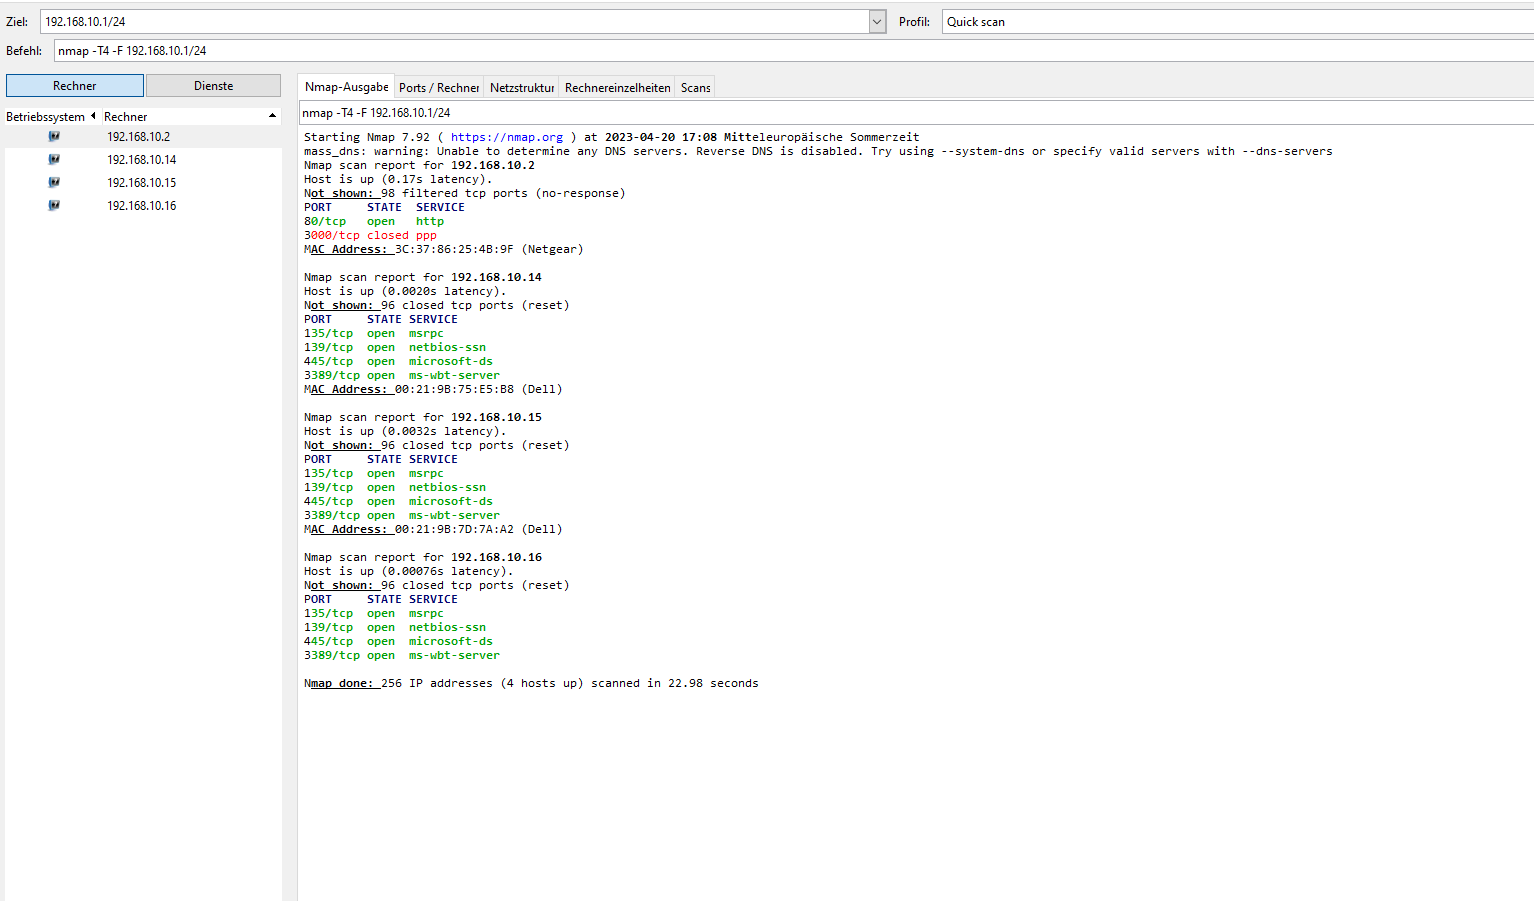
\includegraphics[width=\linewidth]{images/Einrichtung Layer2-Switche/ServerVLAN10Client16.png}
                \caption{Verbindungen Client 16}
            \end{subfigure}
        \caption{Verbindungen VLAN10 - Layer2-Switche}
        \end{figure}
        \begin{figure}[H]
        \centering
            \begin{subfigure}{\linewidth}
                \centering
                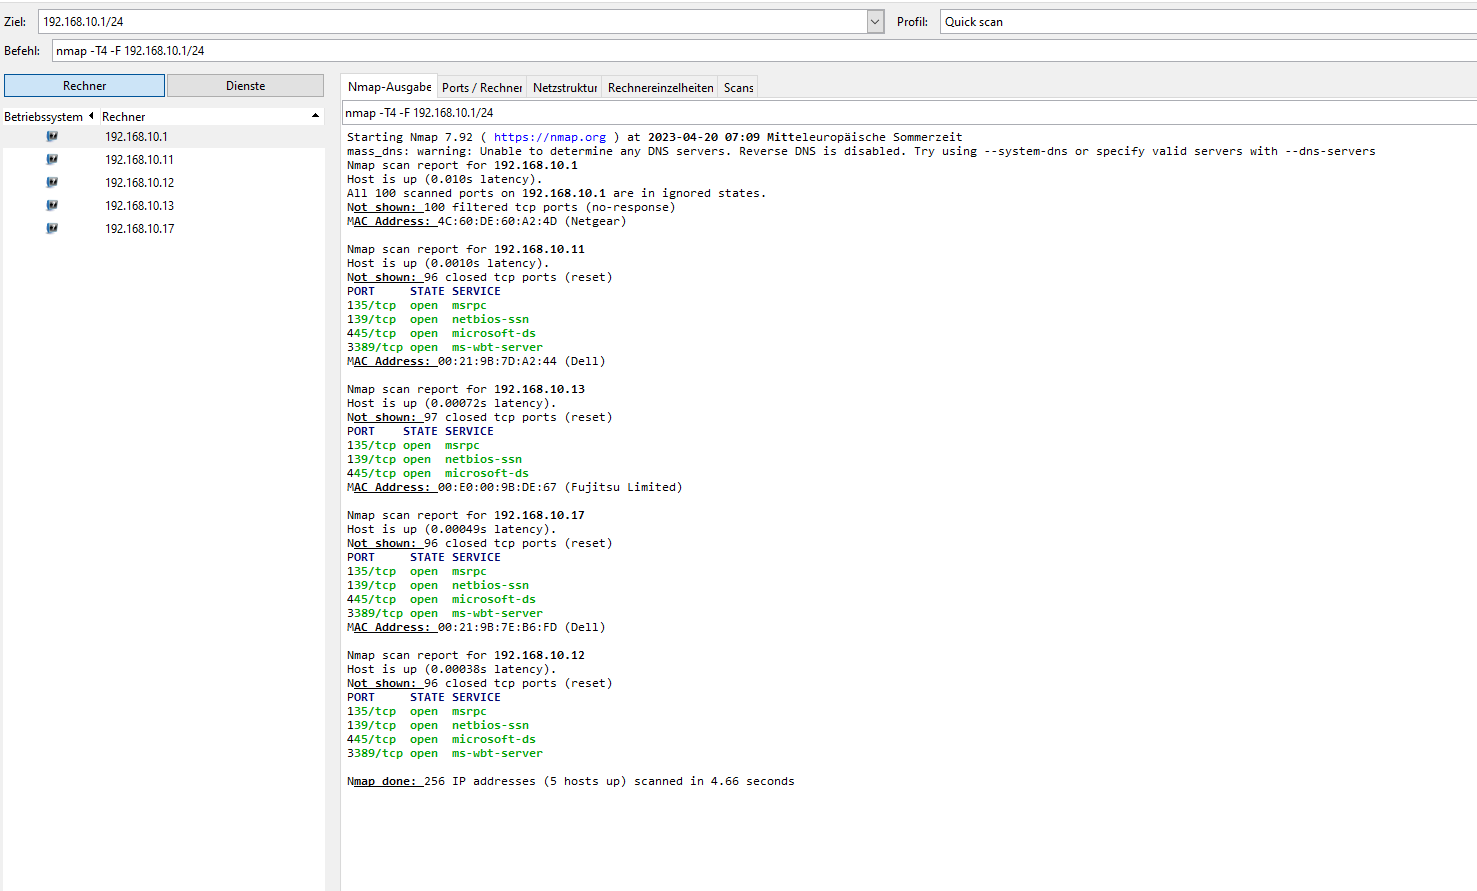
\includegraphics[width=\linewidth]{images/Einrichtung Layer2-Switche/ServerVLAN11Client12.png}
                \caption{Verbindungen Client 12}
            \end{subfigure}
        \caption{Verbindungen VLAN11 - Layer2-Switche}
        \end{figure}%
        \begin{figure}[H]\ContinuedFloat
            \centering
            \begin{subfigure}{\linewidth}
                \centering
                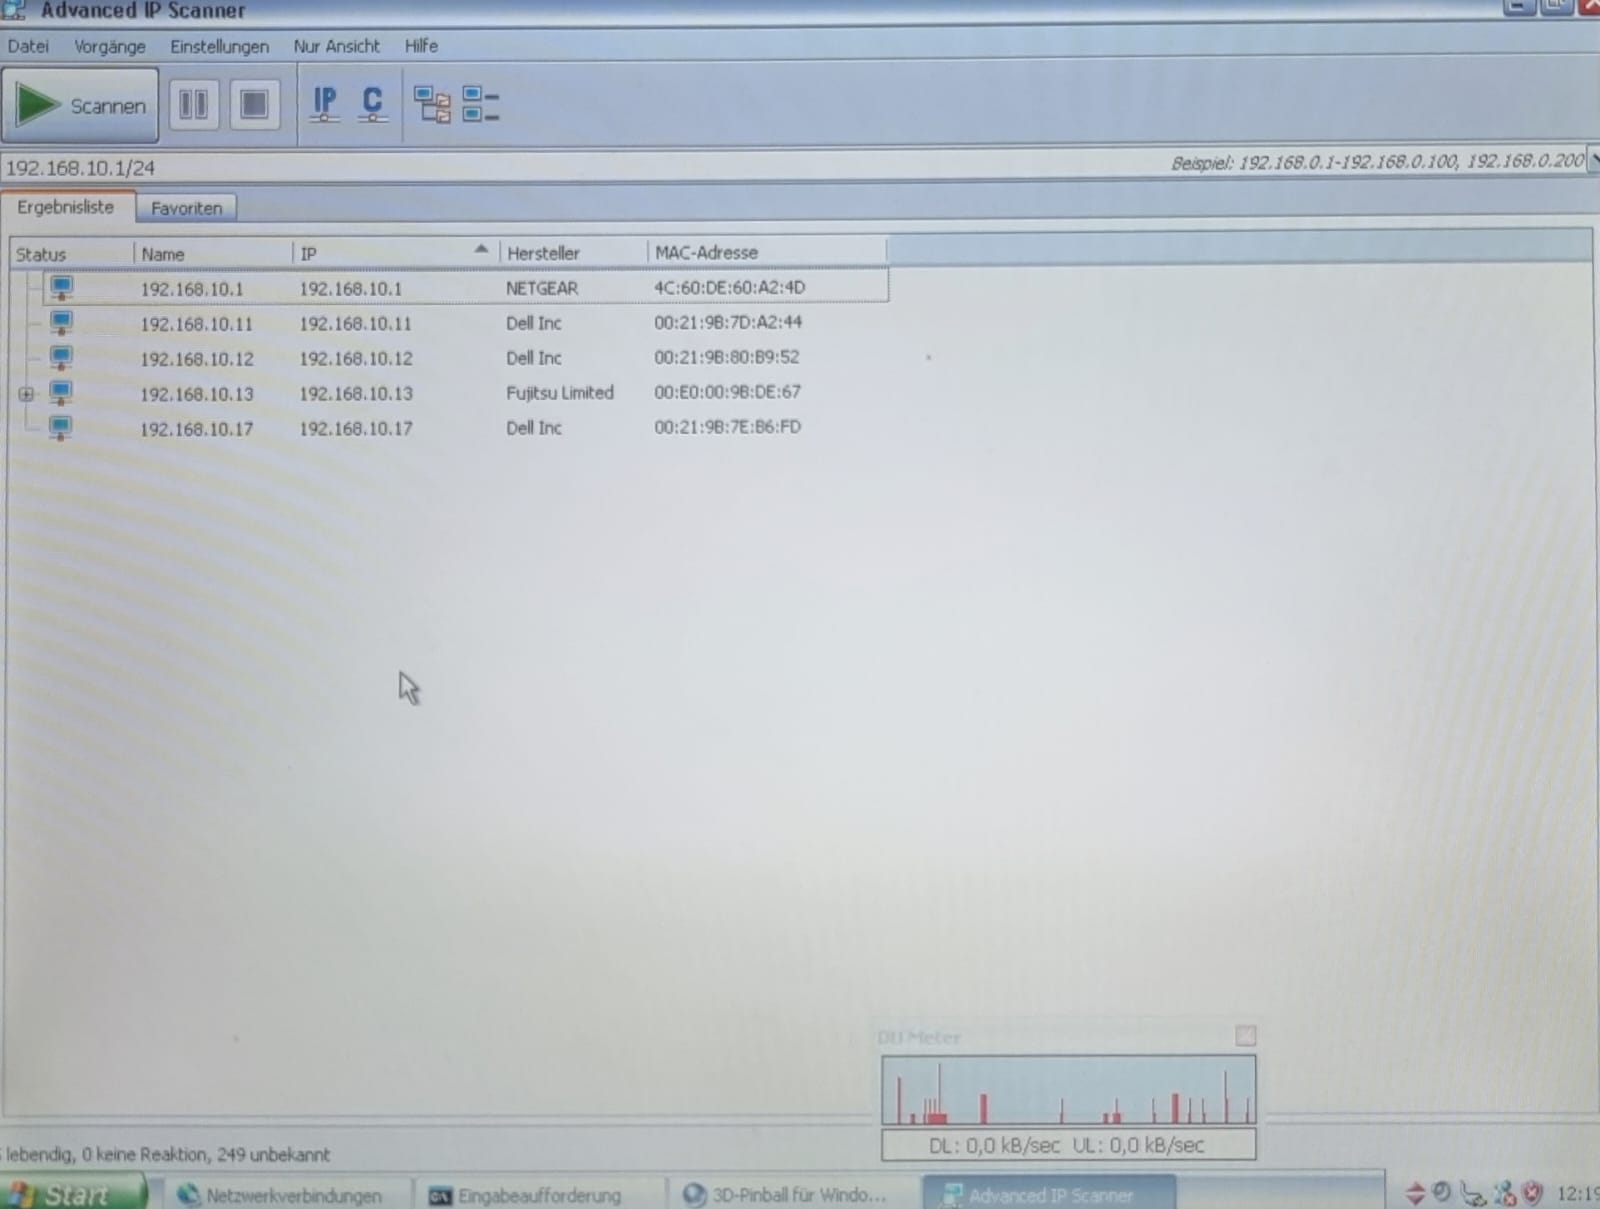
\includegraphics[width=\linewidth]{images/Einrichtung Layer2-Switche/ServerVLAN11Client13.jpg}
                \caption{Verbindungen Client 13}
            \end{subfigure}
            \begin{subfigure}{\linewidth}
                \centering
                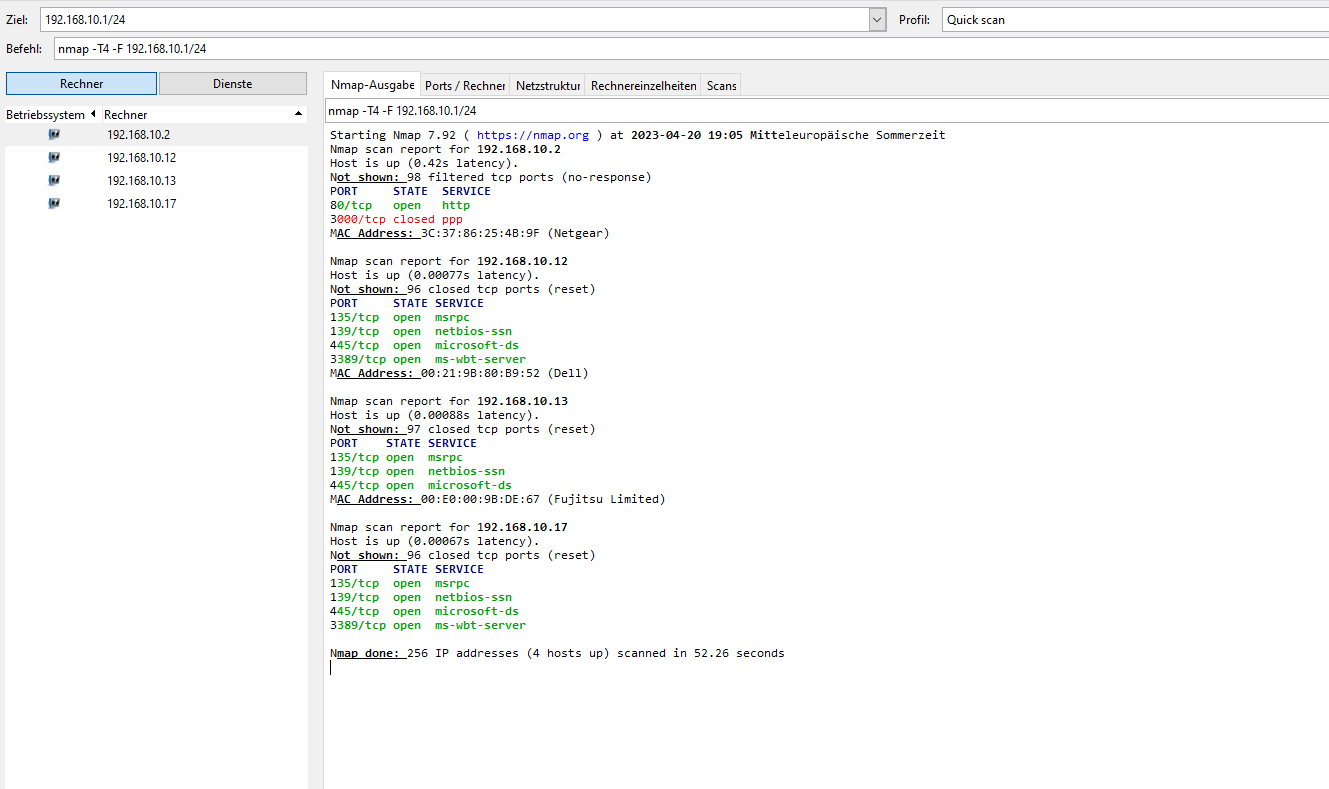
\includegraphics[width=\linewidth]{images/Einrichtung Layer2-Switche/ServerVLAN11Client17.png}
                \caption{Verbindungen Client 17}
            \end{subfigure}
        \caption{Verbindungen VLAN11 - Layer2-Switche}
        \end{figure}





    
\newpage
\section{Auswertung}

    \subsection{Grundlagen Switchkonfiguration}
    
    \newpage
    \subsection{Vergleich und Beurteilung}
    
    \begin{figure}[ht]
        \centering
        
\includegraphics[scale=0.6]{bszet-lgo.png}
        \caption{test}
    \end{figure}

%-------------------------------------------------------------------------------
% Schlussteil
%---------------------------------------------------------------
    \newpage
    \phantomsection
    \addcontentsline{toc}{section}{Literatur}
    \printbibliography

    \newpage
    \addsec{Glossar}

    \newpage
    \phantomsection
    \addcontentsline{toc}{section}{Abbildungsverzeichnis}
    \listoffigures 

    \newpage
    \addsec{Abkürzungsverzeichnis}
    
    \newpage
    \include{EidesstattlicheErklärung}

\end{document}